%package list
\documentclass{article}
\usepackage[top=3cm, bottom=3cm, outer=3cm, inner=3cm]{geometry}
\usepackage{graphicx}
\usepackage{url}
%\usepackage{cite}
\usepackage{hyperref}
\usepackage{array}
%\usepackage{multicol}
\newcolumntype{x}[1]{>{\centering\arraybackslash\hspace{0pt}}p{#1}}
\usepackage{natbib}
\usepackage{pdfpages}
\usepackage{multirow}
\usepackage{multirow}
\usepackage[normalem]{ulem}
\useunder{\uline}{\ul}{}
\usepackage{amsmath}
\usepackage{float}
\usepackage{multicol}
\usepackage{subcaption}


% para tener url cortas en bib
\let\oldUrl\url
\renewcommand{\url}[1]{\href{#1}{Enlace}}
%

%%%%%%%%%%%%%%%%%%%%%%%%%%%%%%%%%%%%%%%%%%%%%%%%%%%%%%%%%%%%%%%%%%%%%%%%%%%%
%%%%%%%%%%%%%%%%%%%%%%%%%%%%%%%%%%%%%%%%%%%%%%%%%%%%%%%%%%%%%%%%%%%%%%%%%%%%
\newcommand{\csemail}{vmachacaa@ulasalle.edu.pe}
%\newcommand{\csdocente}{MSc. Vicente Enrique Machaca Arceda}
\newcommand{\csdocente}{Vicente Machaca Arceda \\ Enzo Velásquez Lobatón \\
	Carlo Corrales Delgado\\
	Oscar Ramirez Valdez
	}
\newcommand{\cscurso}{Computación de Alto Desempeño}
\newcommand{\csuniversidad}{Universidad Nacional de San Agustín de Arequipa}
\newcommand{\csescuela}{Doctorado en Ciencias de la Computación}
\newcommand{\cspracnr}{03}
\newcommand{\cstema}{Inverted index}
%%%%%%%%%%%%%%%%%%%%%%%%%%%%%%%%%%%%%%%%%%%%%%%%%%%%%%%%%%%%%%%%%%%%%%%%%%%%
%%%%%%%%%%%%%%%%%%%%%%%%%%%%%%%%%%%%%%%%%%%%%%%%%%%%%%%%%%%%%%%%%%%%%%%%%%%%


\usepackage[english,spanish]{babel}
\usepackage[utf8]{inputenc}
\AtBeginDocument{\selectlanguage{spanish}}
\renewcommand{\figurename}{Figura}
\renewcommand{\refname}{Referencias}
\renewcommand{\tablename}{Tabla} %esto no funciona cuando se usa babel
\AtBeginDocument{%
	\renewcommand\tablename{Tabla}
}

\usepackage{fancyhdr}
\pagestyle{fancy}
\fancyhf{}
\setlength{\headheight}{30pt}
\renewcommand{\headrulewidth}{1pt}
\renewcommand{\footrulewidth}{1pt}
\fancyhead[L]{\raisebox{-0.2\height}{
\includegraphics[width=3cm]{img/logo_unsa}}}
\fancyhead[C]{}
\fancyhead[R]{\fontsize{7}{7}\selectfont	\csuniversidad \\ \csescuela \\ \textbf{\cscurso} }
\fancyfoot[L]{Vicente, Enzo, Oscar y Carlo}
\fancyfoot[C]{\cscurso}
\fancyfoot[R]{Página \thepage}


% para el codigo fuente
\usepackage{listings}
\usepackage{color}
\definecolor{dkgreen}{rgb}{0,0.6,0}
\definecolor{gray}{rgb}{0.5,0.5,0.5}
\definecolor{mauve}{rgb}{0.58,0,0.82}
\lstset{frame=tb,
	language=Python,
	aboveskip=3mm,
	belowskip=3mm,
	showstringspaces=false,
	columns=flexible,
	basicstyle={\small\ttfamily},
	numbers=none,
	numberstyle=\tiny\color{gray},
	keywordstyle=\color{blue},
	commentstyle=\color{dkgreen},
	stringstyle=\color{mauve},
	breaklines=true,
	breakatwhitespace=true,
	tabsize=3
}


\usepackage{color}

\definecolor{pblue}{rgb}{0.13,0.13,1}
\definecolor{pgreen}{rgb}{0,0.5,0}
\definecolor{pred}{rgb}{0.9,0,0}
\definecolor{pgrey}{rgb}{0.46,0.45,0.48}

\usepackage{listings}
\lstset{language=Java,
  showspaces=false,
  showtabs=false,
  breaklines=true,
  showstringspaces=false,
  breakatwhitespace=true,
  commentstyle=\color{pgreen},
  keywordstyle=\color{pblue},
  stringstyle=\color{pred},
  basicstyle=\ttfamily,
  moredelim=[il][\textcolor{pgrey}]{$$},
  moredelim=[is][\textcolor{pgrey}]{\%\%}{\%\%}
}

\begin{document}
	
	
	
	
\begin{titlepage}
	
	\newcommand{\HRule}{\rule{\linewidth}{0.5mm}} % Defines a new command for the horizontal lines, change thickness here
	
	\center % Center everything on the page
	
	%----------------------------------------------------------------------------------------
	%	HEADING SECTIONS
	%----------------------------------------------------------------------------------------
	
	\textsc{\LARGE \csuniversidad}\\[1.5cm] % Name of your university/college
	\textsc{\Large \cscurso}\\[0.5cm] % Major heading such as course name
	%\textsc{\large Assignment 1}\\[0.5cm] % Minor heading such as course title
	
	%----------------------------------------------------------------------------------------
	%	TITLE SECTION
	%----------------------------------------------------------------------------------------
	
	\vspace{2cm}
	
	\HRule \\[0.4cm]
	{ \huge \bfseries \cstema}\\[0.4cm] % Title of your document
	\HRule \\[1.5cm]
	
	%----------------------------------------------------------------------------------------
	%	AUTHOR SECTION
	%----------------------------------------------------------------------------------------
	
	\begin{minipage}{0.4\textwidth}
		\begin{flushleft} \large
			\emph{Alumnos:}\\
			\csdocente
		\end{flushleft}
	\end{minipage}
	~
	\begin{minipage}{0.4\textwidth}
		\begin{flushright} \large
			\emph{Docente:} \\
			PhD. Alvaro Mamani Aliaga
		\end{flushright}
	\end{minipage}\\[2cm]
	
	% If you don't want a supervisor, uncomment the two lines below and remove the section above
	%\Large \emph{Author:}\\
	%John \textsc{Smith}\\[3cm] % Your name
	
	%----------------------------------------------------------------------------------------
	%	DATE SECTION
	%----------------------------------------------------------------------------------------
	
	{\large \today}\\[2cm] % Date, change the \today to a set date if you want to be precise
	
	%----------------------------------------------------------------------------------------
	%	LOGO SECTION
	%----------------------------------------------------------------------------------------
	
	
\includegraphics[width=100px, keepaspectratio]{img/unsa}\\[1cm] % Include a department/university logo - this will require the graphicx package
	
	%----------------------------------------------------------------------------------------
	
	\vfill % Fill the rest of the page with whitespace
	
\end{titlepage}	
	
	
	

	
	
\tableofcontents
\newpage	
	

	
		
	
\section{Introducción}
	
En Ciencias de la Computación, un Índice Invertido (también conocido como archivo de anuncios o archivo invertido) \cite{indice_invertido} es un estructura de datos de índice que almacena contenido, como palabras, números o documentos, en una base de datos. El propósito de un índice invertido es permitir la búsqueda rápido de texto en los documentos, a un mejor costo de procesamiento cuando los documentos se agregan a la base de datos. El archivo invertido es la estructura de datos más popular utilizada en recuperación de información, \cite{10.1145/296854.277632} utilizado en gran escala por ejemplo en motores de búsqueda. Varios importantes generales mainframe-base sistemas de gestión de base de datos han utilizado las arquitecturas lista de índice invertido, incluyendo ADABAS, DATACOM/DB, y Modelo 204.

Los índices invertidos son la estructura de datos más utilizada en los sistemas de recuperación de información, en particular en aquellos con grandes volúmenes de datos a manejar como los motores de búsqueda; hacen uso eficiente de la idea principal de la matriz de incidencias vista previamente
\newline

Hay dos variantes principales de índices invertidos: \cite{knuth1997art}

\begin{enumerate}
\item A nivel de récord de índice invertido (o índice de archivo invertido o simplemente archivo invertido) contiene una lista de referencias a los documentos de cada palabra. 
\item A nivel de palabra de índice invertido (o completo índice invertido o lista invertida) además contiene las posiciones de cada palabra dentro de un documento.  \cite{baeza1999modern}
\end{enumerate}
La última forma ofrece más funcionalidad, como buscar frases, pero necesita más potencia de procesamiento y espacio para crear. \cite{luk2007efficient}

\subsection{Por qué se llama ``índice invertido''?}
A diferencia de lo que sucede en una base de datos tipo SQL, donde el índice ha sido definido a priori, en el índice invertido el índice se crea a posteriori, cuando el motor ha analizado los documentos sobre los que se basará la búsqueda.

\section{Ejemplo}

Dado los documentos texto:

\begin{itemize}
\item T[0] = ``Esto que es''
\item T[1] = ``Qué es esto'' 
\item T[2] = ``Esto es una banana''
\end{itemize}

Tenemos el siguiente índice de archivo invertido, en donde los enteros se refieren a los índices (o llaves) de los símbolos del documento de texto, T[0], T[1] y T[2]:

\begin{itemize}
    \item ``una'': 	\{2\} 
\item ``banana'': 	\{2\} 
\item ``es'': 		\{0, 1, 2\} 
\item ``esto'': 	\{0, 1, 2\} 
\item ``que'': 	\{0, 1\}
\end{itemize}

Búsqueda de palabras repetidas para ``qué'', ``es'' y ``eso'' daría el conjunto, ejemplo:

\begin{itemize}
    \item ``qué'':  	\{0, 1\}
 \item``es'': 		\{0, 1, 2\}
 \item ``eso'' 	\{0, 1, 2\} 
\end{itemize}

Las palabras se repiten en los documentos de textos \{0,1\}.

Con los mismos textos, obtenemos el siguiente índice invertido, donde los pares indican el número de documento de texto y la posición. Como el índice de los textos y la posición dentro del texto comienzan con cero, el resultado sería el siguiente por ejemplo: ''banana``: \{(2, 3)\} significa que la palabra ''banana`` está en el tercer documento de texto (T[2]), y es la cuarta palabra en ese documento (posición 3).

\begin{itemize}
\item ``una'': 	\{(2, 2)\} 
\item ``banana'': 	\{(2, 3)\} 
\item ``es'': 		\{(0, 1), (0, 4), (1, 1)(2, 1)\} 
\item ``esto'': 	\{(0, 0), (0, 3), (1, 2)(2, 0)\} 
\item ``qué'': 	\{(0, 2), (1, 0)\}
\end{itemize}

Si realizamos la búsqueda de una frase: ``Qué es esto'', se realiza de la misma forma. 


\section{Aplicaciones}

La estructura de datos de índice invertido es un componente central de un típico algoritmo de búsqueda del motor de indexación. Una meta de la implementación del motor de búsqueda es optimizar la velocidad de la consulta: Encontrar los documentos donde se encuentra la palabra X. El  índice avanza por cada documento de texto y por cada palabra y almacena las listas de palabras por cada documento, luego recorre a la inversa para desarrollar un índice invertido. Primero consulta el índice que avanza de inicio a fin la cual recorre la información de forma secuencial a través de cada documento y cada palabra para verificar una coincidencia o palabras repetidas. El tiempo, la memoria y recursos de procesamiento para realizar estas consultas no siempre son técnicamente realistas. En lugar de la lista de las palabras por cada documento en el índice inicial, desarrolla la estructura de datos de índice invertido que enumera los documentos por palabra. Con el índice invertido creado, se puede saltar a la identificación de la palabra (a través de acceso aleatorio). \cite{salton1983extended}

Se puede utilizar para buscar información en los libros, es decir, buscar las concordancias de palabras en los libros importantes que fueron montadas manualmente. Estos fueron los índices efectivamente invertidos con una pequeña cantidad de comentario de acompañamiento que requiere una enorme cantidad de esfuerzo para producir.

En Bioinformática, índices invertidos son muy importantes en la Ensamble de secuencia de fragmentos cortos de ADN secuenciado. Una manera de encontrar la fuente de un fragmento es buscar contra una secuencia de ADN de referencia. Un pequeño número de desajustes (debido a las diferencias entre el ADN y referencia ADN secuenciado, o errores) puede ser contabilizado dividiendo el fragmento en fragmentos más pequeños — por lo menos un subfragmento es probable que coincida con la referencia de secuencia de ADN. El juego requiere construir un índice invertido de todos subcadenas de una cierta longitud de la secuencia de ADN de referencia. Puesto que el ADN humano contiene más de 3 billones de pares de bases, y tenemos que guardar una subcadena de ADN para cada índice y un entero de 32 bits para índice de sí mismo, el requisito de almacenamiento para este índice invertido probablemente sería de decenas de gigabytes. \cite{programmer_click}

\section{Implementación}

\subsection{Ambiente de desarrollo}
Se ha trabajado con las siguientes herramientas y versiones:
\begin{itemize}
    \item Hadoop 3.3.1
    \item Java 11
    \item Maven 3.6.3
\end{itemize}

Haddop, se instaló localmente en una computadora de escritorio, y se utilizó para evaluar la implementación del algoritmo de indice invertido.

%%%%%%%%%%%%%%%%%%%%%%%%%%%%%%%%%%%%%%%%%%%%%%%%%%%%%%%%%%%%%%%%%
%%%%%%%%%%%%%%%%%%%%%%%%%%%%%%%%%%%%%%%%%%%%%%%%%%%%%%%%%%%%%%%%%
%%%%%%%%%%%%%%%%%%%%%%%%%%%%%%%%%%%%%%%%%%%%%%%%%%%%%%%%%%%%%%%%%
%%%%%%%%%%%%%%%%%%%%%%%%%%%%%%%%%%%%%%%%%%%%%%%%%%%%%%%%%%%%%%%%%

\subsection{Código fuente}


\textbf{InvertedIndexDriver}: Este es el archivo principal, encargado de coordinar al \textit{Mapper} y \textit{Reducer}.

\begin{lstlisting}
package org.apache.hadoop.examples;

//hadoop jar target/inverted_index_java-1.0-SNAPSHOT.jar org.apache.hadoop.examples.InvertedIndexDriver input output stopwords.txt

import java.net.URI;

import org.apache.hadoop.conf.Configuration;
import org.apache.hadoop.conf.Configured;
import org.apache.hadoop.fs.FileSystem;
import org.apache.hadoop.fs.Path;
import org.apache.hadoop.io.Text;
import org.apache.hadoop.mapreduce.Job;
import org.apache.hadoop.mapreduce.lib.input.FileInputFormat;
import org.apache.hadoop.mapreduce.lib.input.TextInputFormat;
import org.apache.hadoop.mapreduce.lib.output.FileOutputFormat;
import org.apache.hadoop.util.GenericOptionsParser;
import org.apache.hadoop.util.Tool;
import org.apache.hadoop.util.ToolRunner;
import org.apache.log4j.Logger;

public class InvertedIndexDriver extends Configured implements Tool {

	private static final Logger LOG = Logger
			.getLogger(InvertedIndexDriver.class);

	public static void main(String args[]) throws Exception {
		ToolRunner.run(new InvertedIndexDriver(), args);
	}

	@Override
	public int run(String[] args) throws Exception {
		Configuration conf = new Configuration();
		String[] other_args = new GenericOptionsParser(conf, args).getRemainingArgs();
		if (other_args.length < 2) {
			System.err.println("Error en los argumentos");
			System.exit(2);
		}

		Job job = Job.getInstance(getConf());

		for (int i = 0; i < args.length; i += 1) {
			if ("-skip".equals(args[i])) {
				job.getConfiguration().setBoolean("wordcount.skip.patterns",true);
				i += 1;				
			}
		}
		job.setJarByClass(InvertedIndexDriver.class);

		job.setMapperClass(InvertedIndexMapper.class);
		job.setReducerClass(InvertedIndexReducer.class);

		job.setInputFormatClass(TextInputFormat.class);
		job.setMapOutputKeyClass(Text.class);
		job.setMapOutputValueClass(Text.class);

		job.setOutputKeyClass(Text.class);
		job.setOutputValueClass(Text.class);

		Path inputFilePath = new Path(args[0]);
		Path outputFilePath = new Path(args[1]);

		FileInputFormat.addInputPath(job, inputFilePath);
		FileOutputFormat.setOutputPath(job, outputFilePath);

		FileSystem fs = FileSystem.newInstance(getConf());

		if (fs.exists(outputFilePath)) {
			fs.delete(outputFilePath, true);
		}

		job.waitForCompletion(true);
		return 0;
	}
}
\end{lstlisting}

\textbf{InvertedIndexMapper}, es el encargado de leer la entrada (directorio con palabras a buscar y contar). Cabe mencionar que no va a considerar las palabras del archivo \textit{stopwords.txt}. \\
\begin{lstlisting}
package org.apache.hadoop.examples;

import java.io.BufferedReader;
import java.io.IOException;
import java.io.InputStreamReader;
import java.net.URI;
import java.util.HashSet;
import java.util.Set;
import java.util.StringTokenizer;

import org.apache.hadoop.conf.Configuration;
import org.apache.hadoop.fs.FSDataInputStream;
import org.apache.hadoop.fs.FileSystem;
import org.apache.hadoop.fs.Path;
import org.apache.hadoop.io.LongWritable;
import org.apache.hadoop.io.Text;
import org.apache.hadoop.mapreduce.Mapper;
import org.apache.hadoop.mapreduce.lib.input.FileSplit;
import org.apache.log4j.Logger;

public class InvertedIndexMapper extends Mapper<LongWritable, Text, Text, Text> {

	private static final Logger LOG = Logger.getLogger(InvertedIndexMapper.class);

	Set<String> stopwords = new HashSet<String>();
	Text word = new Text();

	@Override
	protected void setup(Context context) throws IOException {
		Configuration conf = context.getConfiguration();

		LOG.info("Leemos");

		if (conf.getBoolean("wordcount.skip.patterns", false)) {
			URI[] localPaths = context.getCacheFiles();
			Path path = new Path(localPaths[0]);

			LOG.info("Procesamos:" + path);

			try {
				FileSystem fs = FileSystem.get(context.getConfiguration());
				FSDataInputStream in = fs.open(path);
				BufferedReader br = new BufferedReader(new InputStreamReader(in));
				String pattern;

				LOG.info("stopword a hash");
				while ((pattern = br.readLine()) != null) {
					stopwords.add(pattern);
				}
			} catch (IOException ioe) {
				System.err.println("Error '" + path);
			}
		}
	}

	public void map(LongWritable key, Text value, Context context)
			throws IOException, InterruptedException {
		String fileName = ((FileSplit) context.getInputSplit()).getPath().getName();
		String line = value.toString().replaceAll("[^\\w\\s]|('s|ly|ed|ing|ness|.|,|\\?|'|:|;) ", " ").toLowerCase();

		StringTokenizer tokenizer = new StringTokenizer(line);
		while (tokenizer.hasMoreTokens()) {
			String wordText = tokenizer.nextToken();
			if (stopwords.contains(wordText))
				continue;
			word.set(wordText);
			context.write(word, new Text(fileName));
		}
	}
}

\end{lstlisting}

\textbf{InvertedIndexReducer}: Lee las \textit{tuplas} (word, lista de archivos donde aparece), del \textit{mapper}. Aquí, se utiliza una tabla hash para contar la cantidad de ocurrencias de cada palabra.\\
\begin{lstlisting}
package org.apache.hadoop.examples;

import java.io.IOException;
import java.util.HashMap;

import org.apache.hadoop.io.Text;
import org.apache.hadoop.mapreduce.Reducer;

public class InvertedIndexReducer extends Reducer<Text, Text, Text, Text> {
	public void reduce(Text key, Iterable<Text> values, Context context) throws IOException, InterruptedException {
		StringBuilder stb = new StringBuilder();
		HashMap<String, Integer> file_freq = new HashMap<String, Integer>();

		for (Text val : values) {
			Integer count = file_freq.get(val.toString());
			if (count == null) {
				count = 0;
			}
			file_freq.put(val.toString(), count + 1);
		}
		context.write(key, new Text(file_freq.toString()));
	}
}

\end{lstlisting}



%%%%%%%%%%%%%%%%%%%%%%%%%%%%%%%%%%%%%%%%%%%%%%%%%%%%%%%%%%%%%%%%%
%%%%%%%%%%%%%%%%%%%%%%%%%%%%%%%%%%%%%%%%%%%%%%%%%%%%%%%%%%%%%%%%%
%%%%%%%%%%%%%%%%%%%%%%%%%%%%%%%%%%%%%%%%%%%%%%%%%%%%%%%%%%%%%%%%%
%%%%%%%%%%%%%%%%%%%%%%%%%%%%%%%%%%%%%%%%%%%%%%%%%%%%%%%%%%%%%%%%%

\section{Resultados}
El código fuente descrito anteriormente, fue compilado y se genero un \textit{jar}: ``inverted\_index\_java-1.0-SNAPSHOT''. Este \textit{jar}, será utilizado por hadoop.\\

El \textit{input} de la aplicación son tres archivos, ambos con diferentes palabras. Los archivos son:

\begin{itemize}
    \item input1.txt
    \item input2.txt
    \item imput3.txt
\end{itemize}

Por ejemplo, el contenido del archivo \textit{input3.txt} es:
\begin{lstlisting}
la universidad nacional, la universidad privada
Este es un archivo con palabra, para evaluar el algoritmo inverted index
\end{lstlisting}

\vspace{0.25cm}

Luego, en las Figuras \ref{fig:hadoop} y \ref{fig:hadoop2}, se muestra un extracto de la ejecución de la aplicación en Hadoop. 

\begin{figure}[H]
    \centering
    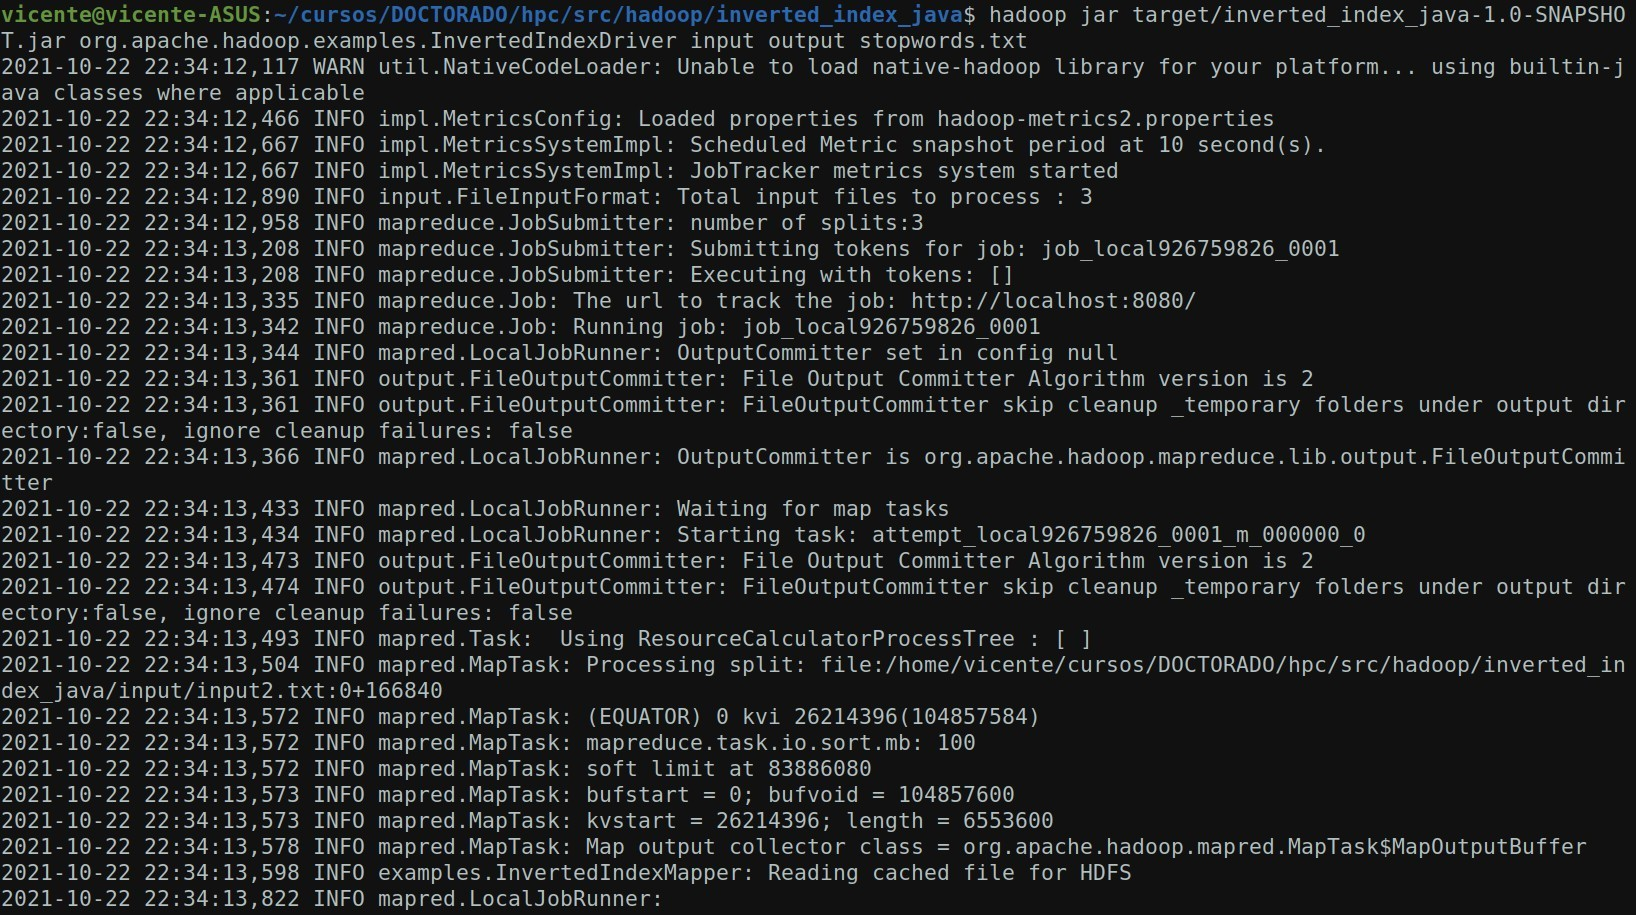
\includegraphics[width=15cm]{tareas/img/hadoop.jpg}
    \caption{Ejecución del proyecto en Hadoop.}
    \label{fig:hadoop}
\end{figure}

\begin{figure}[H]
    \centering
    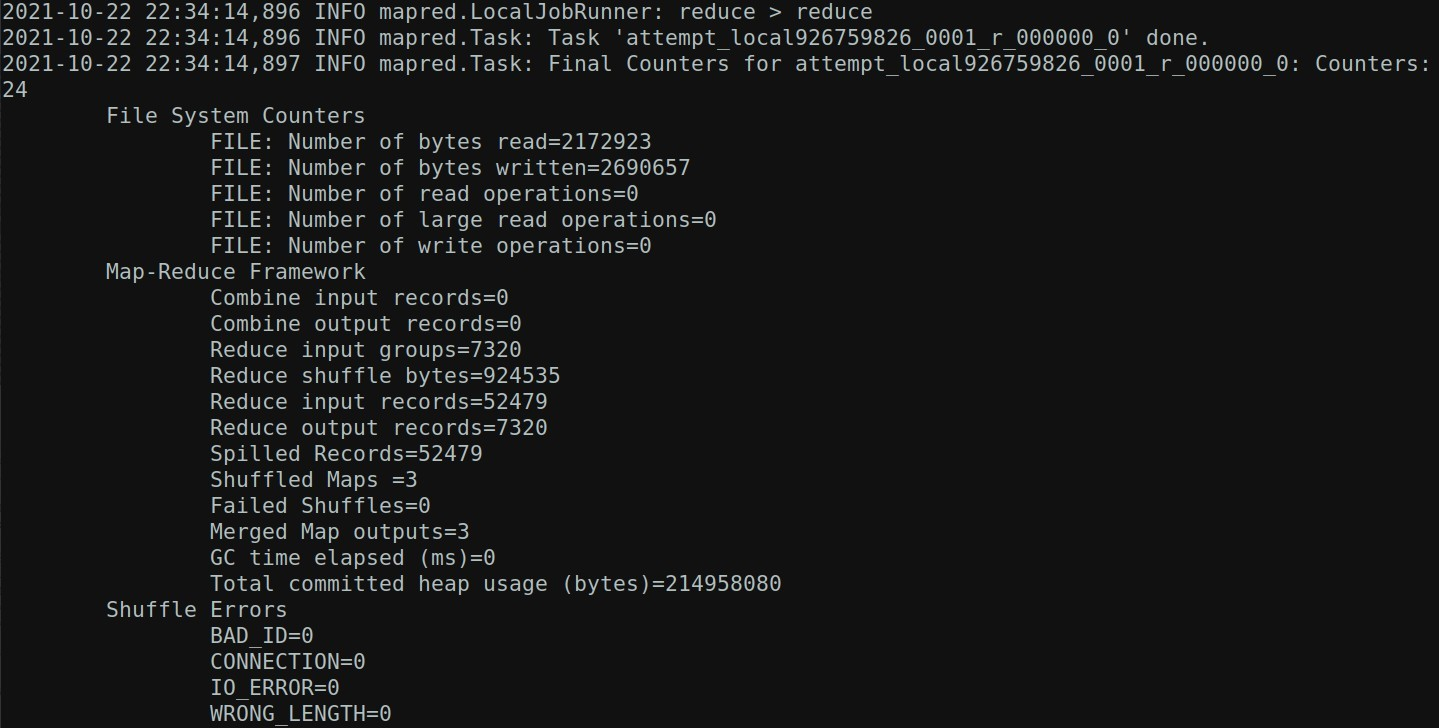
\includegraphics[width=15cm]{tareas/img/hadoop2.jpg}
    \caption{Ejecución del proyecto en Hadoop.}
    \label{fig:hadoop2}
\end{figure}


Finalmente se genera la salida, esta contiene \textit{tuplas} de cada palabra, la ubicación y la cantidad de palabras encontradas. Por ejemplo, aquí mostramos un extracto de la salida:

\begin{lstlisting}
...
understand	{input1.txt=1, input2.txt=1}
unified	{input1.txt=1, input2.txt=1}
unit	{input1.txt=3, input2.txt=3}
universida	{input3.txt=2, input2.txt=1}
universit	{input1.txt=1, input2.txt=1}
university	{input1.txt=5, input2.txt=5}
unles	{input1.txt=2, input2.txt=2}
unpac	{input1.txt=1, input2.txt=1}
...
\end{lstlisting}

Aquí, verificamos que encontro la palabra ``universida'', dos veces en el archivo \textit{input3.txt}, y una vez en el archivo \textit{input2.txt}



\bibliographystyle{apalike}
%\bibliographystyle{IEEEtranN}
\bibliography{bibliography}

	
	
	
	
\end{document}